\documentclass[11pt]{article}

\usepackage[norsk]{babel}
\usepackage[utf8]{inputenc}
\usepackage{amsmath, amssymb, amsthm}
\usepackage{graphicx, float}
\usepackage{pstricks-add}


\author{Kjetil Kjeka}
\title{TTK4130 - Exercise 1}
\date{\today}


%Slik at matriser kan defineres med linjer
\makeatletter
\renewcommand*\env@matrix[1][*\c@MaxMatrixCols c]{%
  \hskip -\arraycolsep
  \let\@ifnextchar\new@ifnextchar
  \array{#1}}
\makeatother




\begin{document}
\maketitle
\section*{Problem 1}
\subsection*{a}
Know that:
\[Ni = \phi (R_a + R_c + R_b + R_r) \]
where
\[R_a = \frac{z}{A \mu_0} \]
Under the assumption that $R_c$ and $R_b$ are negligible
\[Ni = \phi (R_a + R_r) \]
And the return path is constant denoted $z_0$
\[R_r = \frac{z_0}{A \mu_0}\]
Meaning the total magnetomotive force can be expressed as:
\[Ni = \phi \frac{z + z_0}{A \mu_0} \]

\subsection*{b}
Given the inductance
\[ L(z) = \frac{N^2 A \mu_0}{z + z_0}\]
We find that
\[ \frac{dL}{dz} = - \frac{N^2 A \mu_0}{(z + z_0)^2} \]
Which gives the magnetic force
\[ F = - \frac{i^2}{2} \frac{N^2 A \mu_0}{(z + z_0)^2} \]
Which agains make the total force on the ball
\[ \sum F = G + F = mg - \frac{i^2}{2} \frac{N^2 A \mu_0}{(z + z_0)^2} \]
Netwons 2. law states
\[ \sum F = m \ddot{z} \]
Combining this gives the following equation of motion
\[\ddot{z} = g - \frac{1}{m} \frac{i^2}{2} \frac{N^2 A \mu_0}{(z + z_0)^2} \]

\subsection*{c}
Our equation is on the form
\[\ddot{z} = f(z, i) \]
A linearization at $(z_d, i_d)$ can then be expressed as
\[\ddot{z} = f(z_d, i_d) + (z - z_d) \frac{df}{dz}\bigg|_{(z_d, i_d)} + (i - i_d) \frac{df}{di}\bigg|_{(z_d, i_d)} \]
where
\[f(z_d, i_d) = g - \frac{i_d^2}{2m} \frac{N^2 A \mu_0}{(z_d + z_0)^2} \]
\[\frac{df}{dz}\bigg|_{(z_d, i_d)} = \frac{i_d^2}{m} \frac{N^2 A \mu_0}{(z_d + z_0)^3} \]
\[\frac{df}{di}\bigg|_{(z_d, i_d)} = -\frac{i_d}{m} \frac{N^2 A \mu_0}{(z_d + z_0)^2} \]
combining equations give the linearized system
\[\ddot{z} = g - \frac{i_d}{m} \frac{N^2 A \mu_0}{(z_d + z_0)^2} \bigg[ \frac{i_d}{2} + (z-z_d)\frac{i_d}{z_d + z_0} - (i - i_d) \bigg] \]


\section*{Problem 2}
\subsection*{b}
For it to fit with the motor model computationaly it needs $\omega_{i-1}$ as input and to fit with next load it needs $\omega_{i}$ as output. It also need to have $T_{i-1}$ as output and $T_i$ as input. For energy flow it would possibly be more natural to have $T_{i-1}$ and $\omega_{i-1}$ as inputs and $T_i$ and $\omega_i$ as outputs.

\subsection*{d}
When simulating it seems like the last load will just increase in speed until infinity. This is not the simulations fault but our simplified motor model without any back-emf or similar.
\begin{figure}[H]
\centering
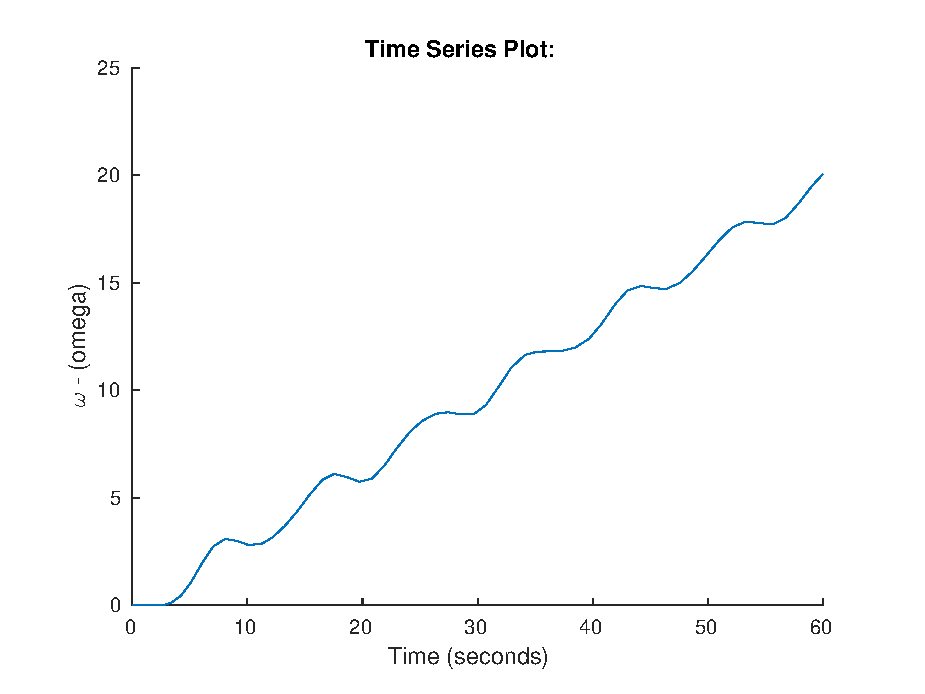
\includegraphics[width=0.8\textwidth]{matlabRotationalSpeed.eps}
\caption{Rotational speed of last load in matlab}
\end{figure}

\subsection*{e}
The most obvious thing to comment is that the system is unstable.
\begin{figure}[H]
\centering
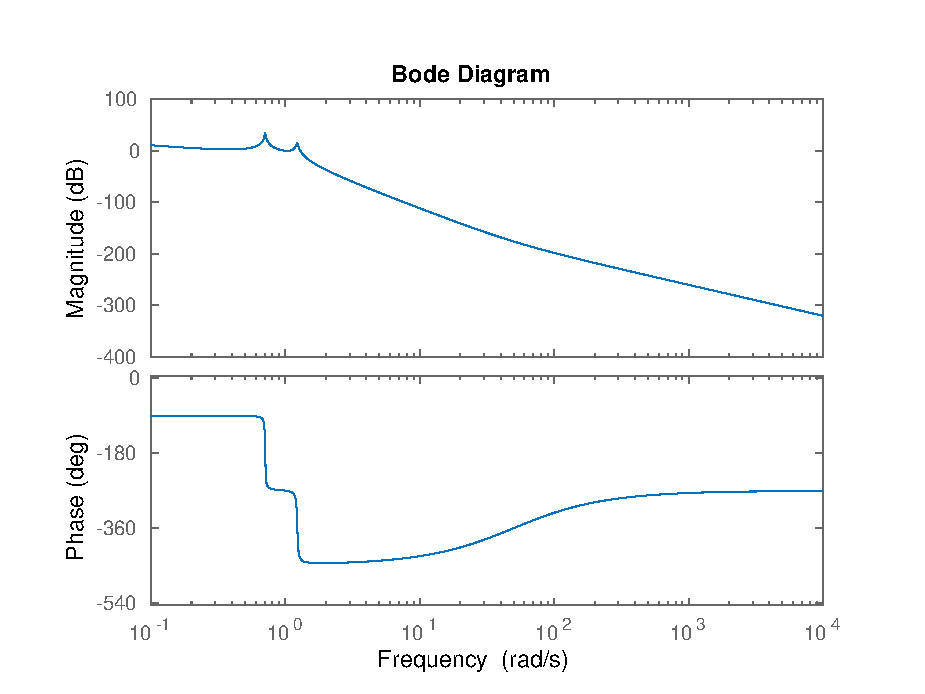
\includegraphics[width=0.8\textwidth]{matlabBode.eps}
\caption{Bode plot done with matlab}
\end{figure}



\section*{Problem 3}
\subsection*{a}
\begin{figure}[H]
\centering
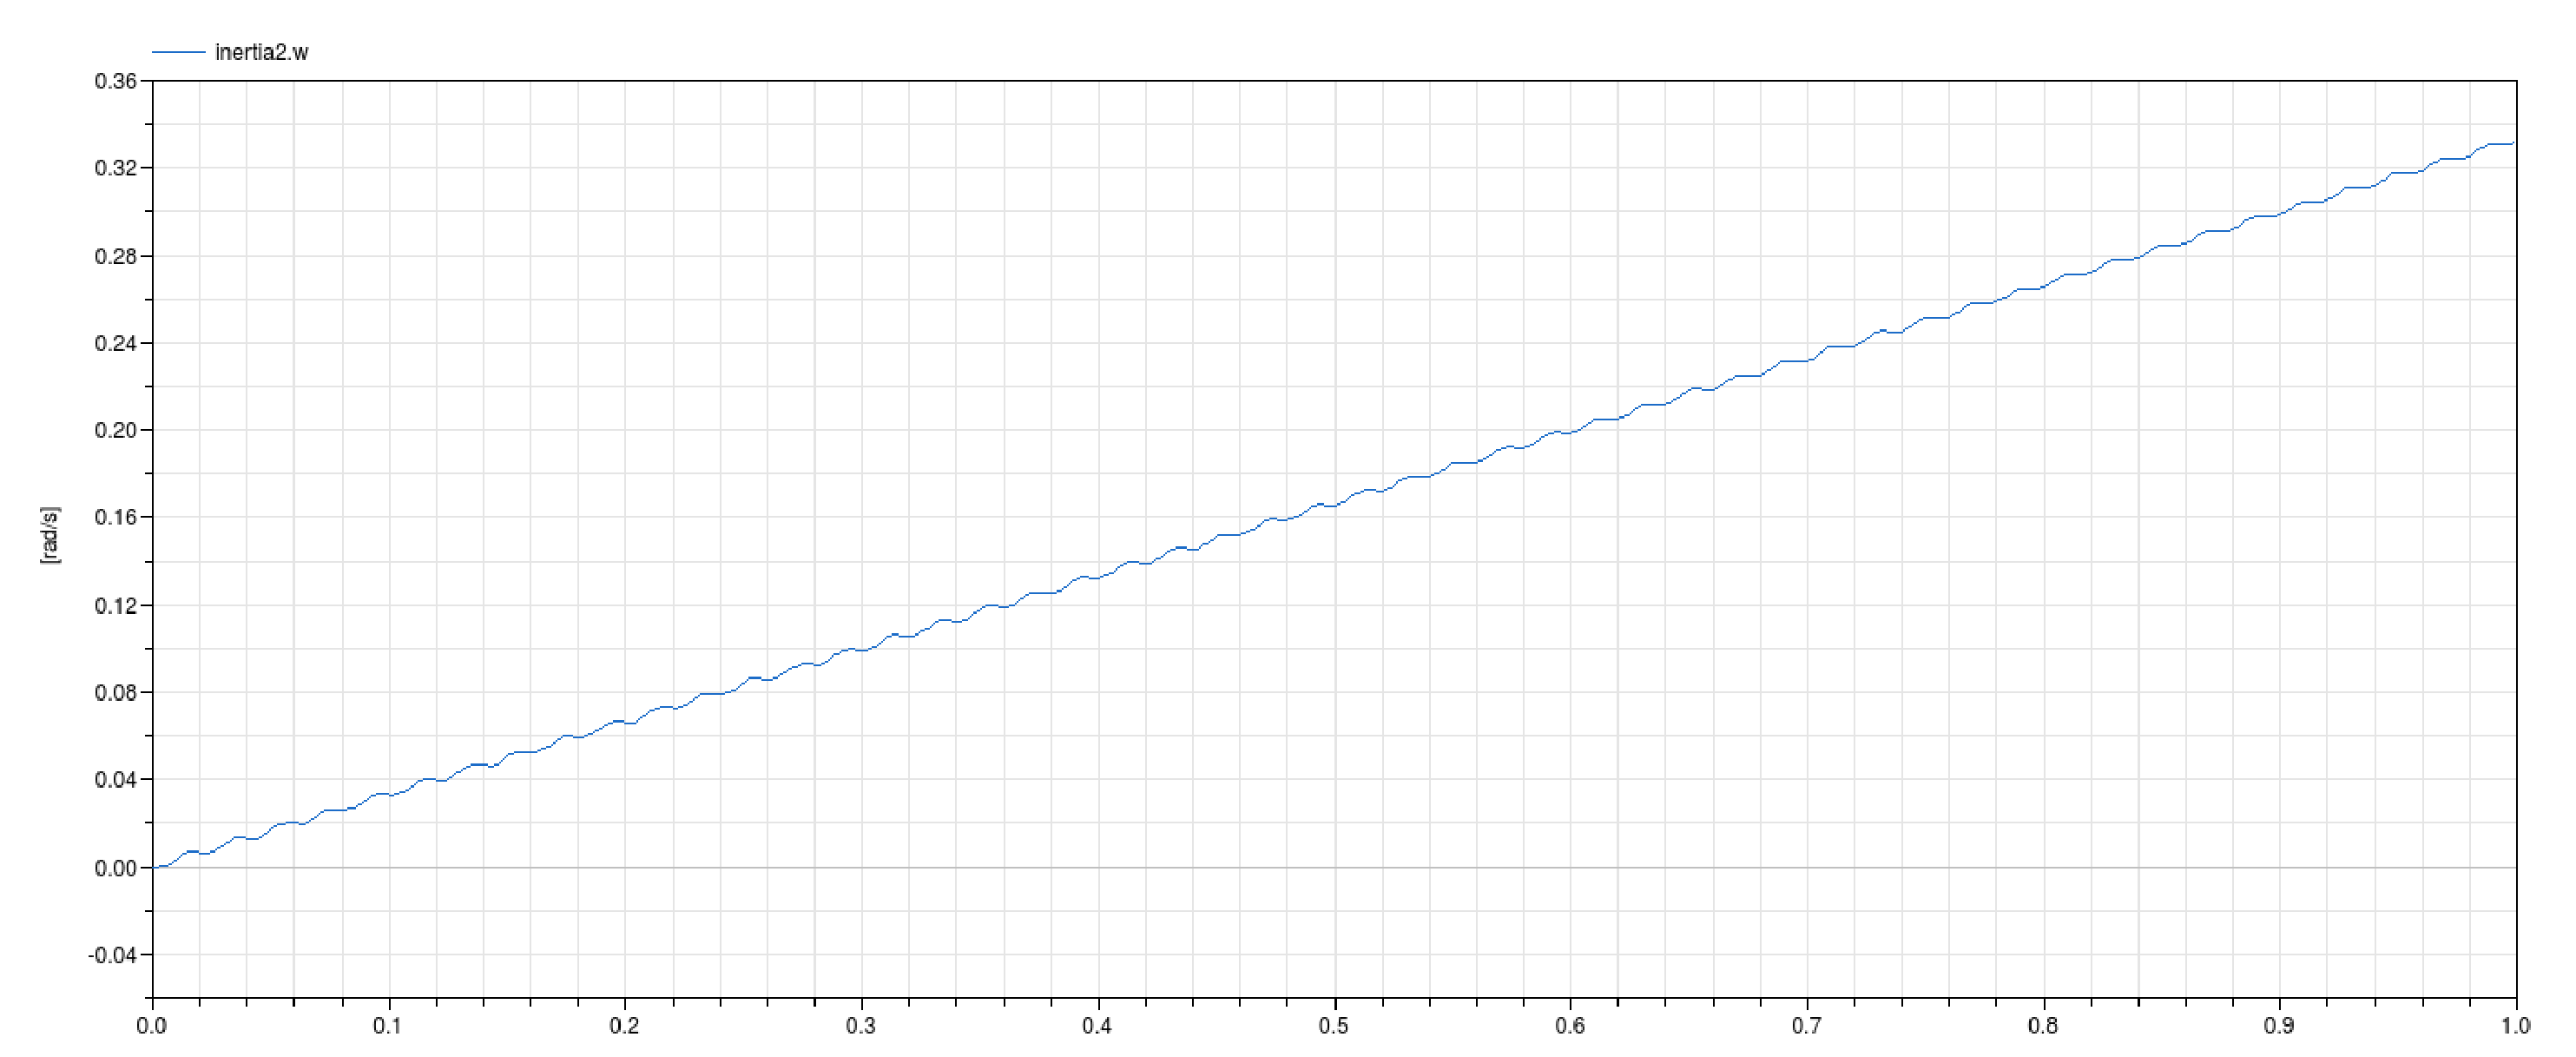
\includegraphics[width=0.8\textwidth]{DymolaRotationalSpeed.eps}
\caption{Rotational speed of last load in dymola}
\end{figure}


\end{document}